\section{The Matrix Keypad}
\label{section:MatrixKeyboard}

The matrix keypad used for the project is the \textit{Matrix Keyboard 4x4 on PCB} from IHA's Embedded Stock \cite{MatrixKeyboard}. It can be seen highlighted in the blue square of figure \ref{ProductComponents}.

For a detailed description of its interface, see table \ref{table:MembraneKeypad} of section \ref{section:InternalBlockDiagram} - \nameref{section:InternalBlockDiagram}.

\subsection{Keypad Driver}
In order to make use of the matrix keypad in the software of our project, we developed a keypad driver. The interface of this driver can be seen in the class diagram of figure \ref{KeypadDriverClassDiagram}.

\begin{figure}[H]
	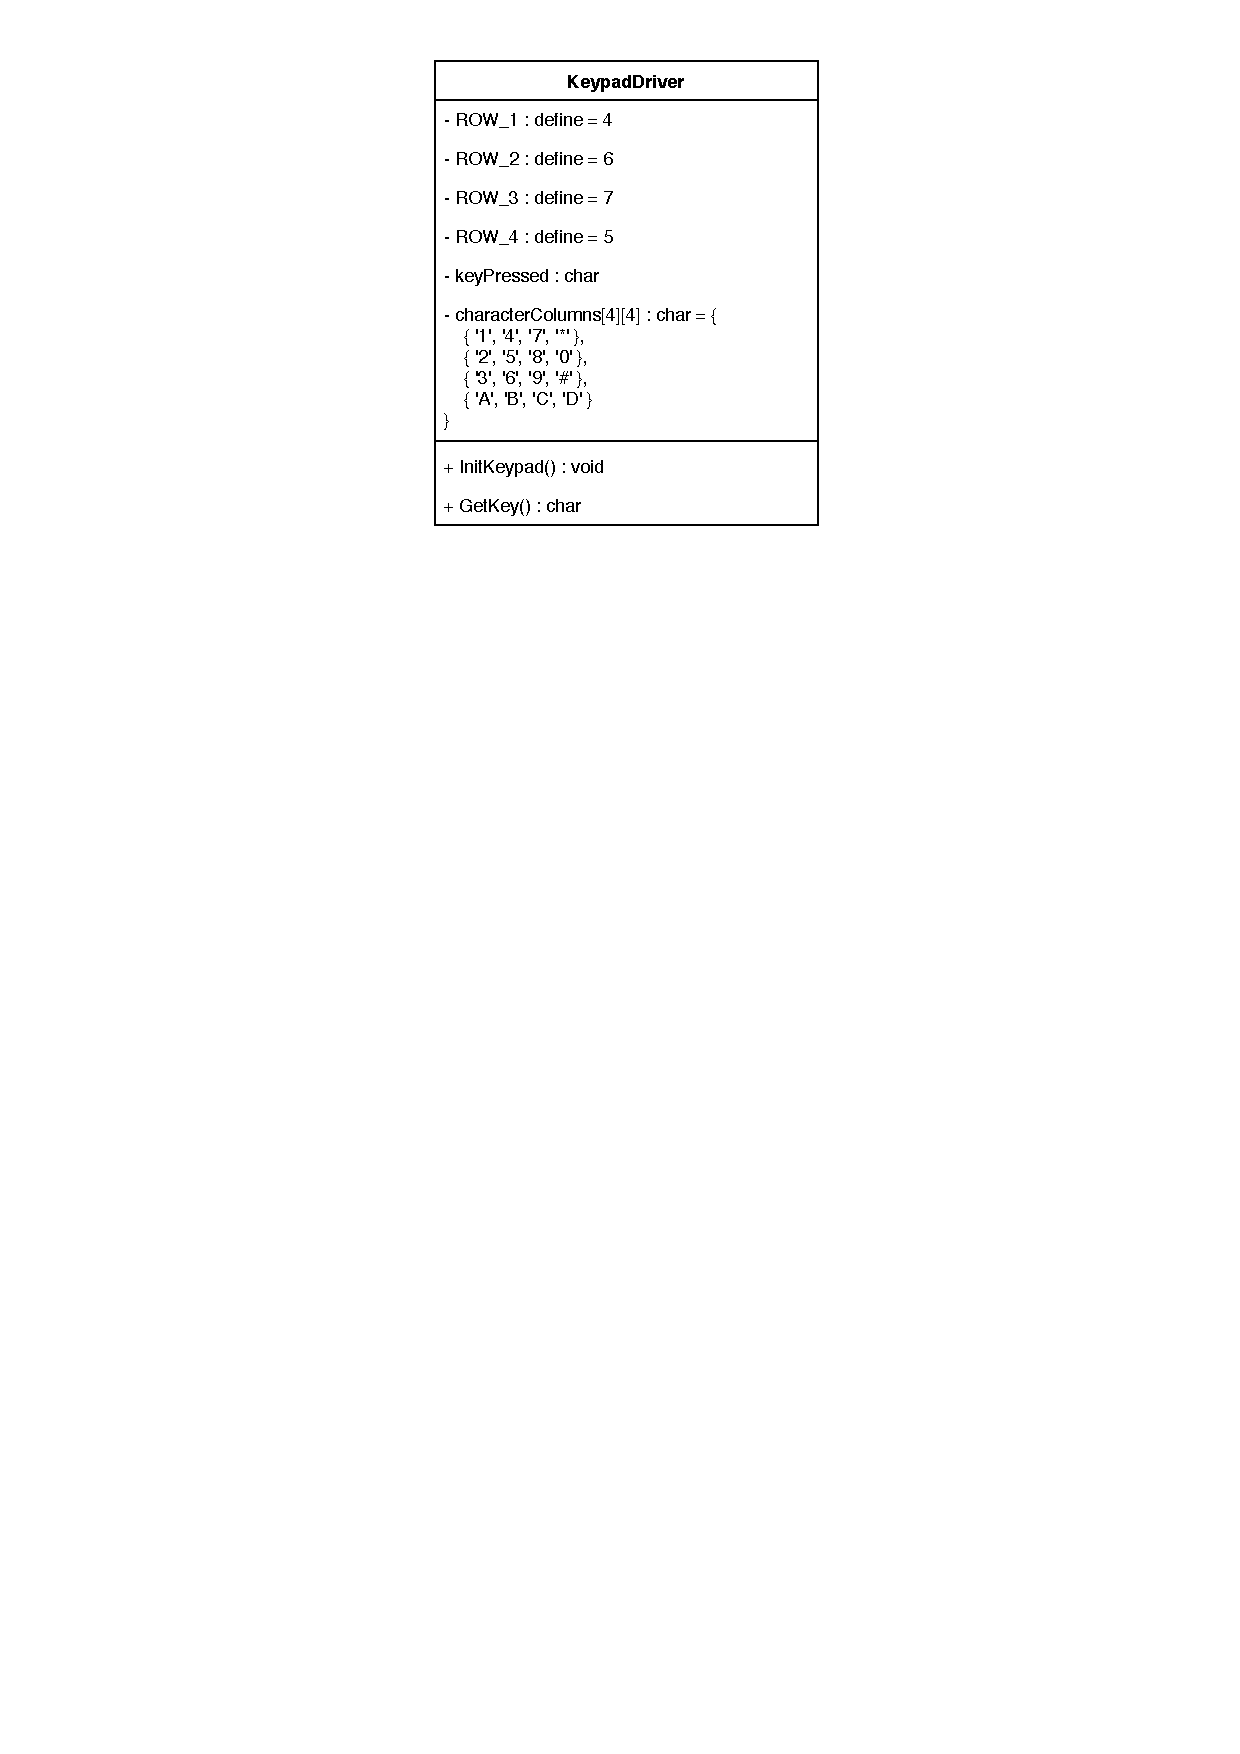
\includegraphics[scale=1.0]{KeypadDriverClassDiagram}
	\centering
	\caption{Class diagram for keypad driver}
	\label{KeypadDriverClassDiagram}
\end{figure}

A description of the methods of the KeypadDriver can be seen in table \ref{table:KeypadDriverMethodDescriptions}.

A description of the attributes of the KeypadDriver can be seen in table \ref{table:KeypadDriverAttributeDescriptions}.

\begin{table}[H]
	\centering
	\begin{tabular}{|l|l|}
		\hline
		Method & Description \\ \hline
		InitKeypad & \begin{tabular}[c]{@{}l@{}}This method initializes specific pins of the Atmega 2560\\ to be input and output, according to the required\\ configuration of the matrix keypad andAtmega2560\\ described in the internal block diagrams of section ...\end{tabular} \\ \hline
		GetKey & \begin{tabular}[c]{@{}l@{}}This method can be called by external clients in order\\ to retrieve the currently held down key of the\\ matrix keypad. What is returned is an ASCII\\ character representation of the character pressed on\\ the keypad.\end{tabular} \\ \hline
	\end{tabular}
	\caption{Descriptions of the methods of the Keypad Driver}
	\label{table:KeypadDriverMethodDescriptions}
\end{table}

\begin{table}[H]
	\centering
	\begin{tabular}{|l|l|}
		\hline
		Attribute & Description \\ \hline
		ROW\_1 - ROW\_4 & \begin{tabular}[c]{@{}l@{}}These defines are simply descriptive names given\\ to the pin numbers used to read the output. They\\ are defined to make the source code easier to read\\ and understand.\end{tabular} \\ \hline
		keyPressed & \begin{tabular}[c]{@{}l@{}}This attribute represents the currently held\\ down key from the keypad. The value of it\\ is what is returned to external clients.\end{tabular} \\ \hline
		characterColumns & \begin{tabular}[c]{@{}l@{}}This is a 2D array, in which each individual array\\ represents a single column of the physical\\ keypad. This array is used by mapping logic to\\ retrieve the correct ASCII character based\\ on the current scan location.\end{tabular} \\ \hline
	\end{tabular}
	\caption{Descriptions of the attributes of the Keypad Driver}
	\label{table:KeypadDriverAttributeDescriptions}
\end{table}

\subsection{Scanning}
The advantage of a matrix keypad is that it is relatively straightforward to determine the character that is currently pressed down on it. The keypad makes no use of communication protocols such as SPI or I2C, thus the system is not complicated further by this. Instead, the keypad consists of input and output signals that can be read and written to through the Atmega2560 registers.

The algorithm we use to determine the currently held down key is called \textit{scanning} \cite{KeypadScanningAlgorithm}. Essentially, we sequentially output a low signal to the pins for each of the keypad columns, and then read the state of the pins for each individual row. 

The sequence of our scanning algorithm implementation can be seen in the sequence diagram of figure \ref{ScanningAlgorithmSequence}. The \textit{main} software component can be read in detail in section \textbf{FUNDOC GAME LOGIC}.

\begin{figure}[H]
	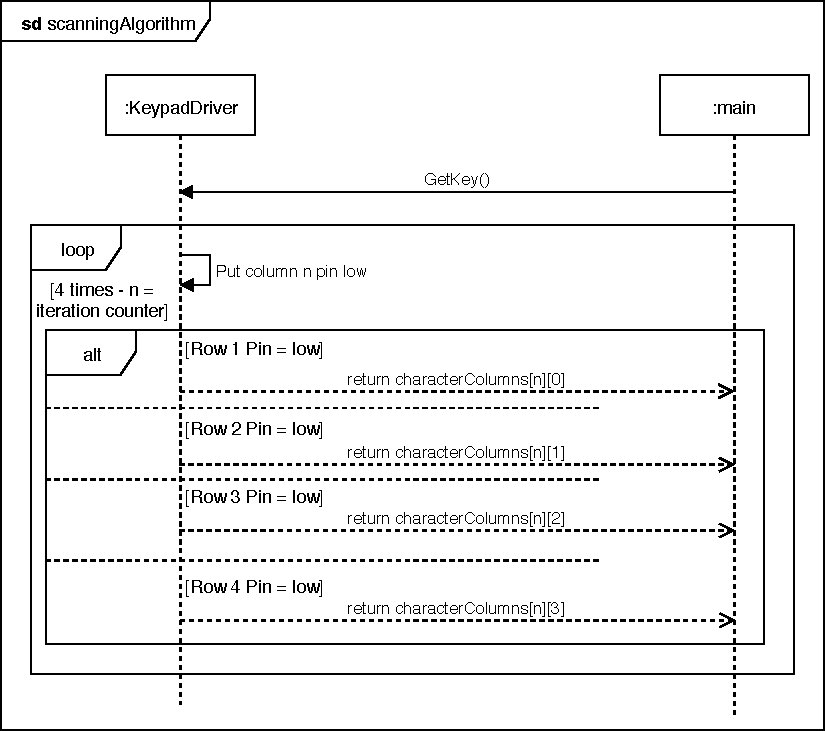
\includegraphics[scale=0.9]{ScanningSequenceDiagram}
	\centering
	\caption{The sequence of the scanning algorithm as implemented in our Keypad Driver.}
	\label{ScanningAlgorithmSequence}
\end{figure}

